\section{Результаты (2)}\label{section:dyck_1}

Вспомним алгоритм~\ref{algo:PI}. Его слабым местом, дающим кубическую нижнюю оценку, было поддержание инкрементального транзитивного замыкания. Проблемы была в том, что рёбра могли добавляться по одному, и тогда никаким более простым/быстрым методом было не справиться. Однако, если новые пути появляются не по-одному, а сразу большими группами, задачу можно решать эффективнее.

\subsection{Алгоритм, основанный на неикрементальном транзитивном замыкании}

Ключом к более быстрому решению является построение транзитивного замыкания с нуля на каждой итерации алгоритма. И, так как обычное транзитивное замыкание можно найти за субкубическое время, то если итераций алгоритма немного, такое решение получается асимптотически быстрее основного (алгоритма~\ref{algo:PI}).

В листинге~\ref{algo:P} приведён псевдокод решения.

\begin{algorithm}[h]
    \floatname{algorithm}{Listing}
    \begin{algorithmic}[1]
    \caption{Алгоритм достижимости для РКА}
    \label{algo:P}
    \Function{RSMReachability}{$\cool{R}$}
        \State{$A \gets$ Adjacency matrix for $\cool{R}$}
        \While{$A$ is changing}
            \State{$A' \gets \textit{transitiveClosure}(A)$}
            \Comment{Построение транзитивного замыкания}
            \For{$i \in 1..k$}
               \For{$u \in En_i$}
                    \For{$v \in Ex_i$}
                        \If{$A'_{u,v} \wedge \overline{A_{u,v}}$}
                            \State{$A' \gets A' \cup getEdges(i, u, v)$}
                            \Comment{Добавление новых рёбер}
                        \EndIf
                    \EndFor
               \EndFor
            \EndFor
            \State{$A \to A'$}
        \EndWhile
    \State \Return $A$
    \EndFunction
    \end{algorithmic}
\end{algorithm}

Изначально, так же, как и в алгоритме~\ref{algo:PI}, в матрицу смежности $A$ записываются все внутренние рёбра РКА $\cool{R}$.

Далее, внешний цикл повторяется, пока матрица смежности $A$ меняется (т.е. пока добавляются новые рёбра). На каждой итерации считается $A'$~--- транзитивное замыкание $A$. После этого находятся все новые пути вида $\langle$стартовое состояние$\rangle$ $\path$ $\langle$конечное состояние$\rangle$~--- те рёбра между стартовой и конечной вершинами компоненты, которых не было в $A$, но которые есть в $A'$~--- и добавляются соответствующие этим путям рёбра.

\subsubsection*{Время работы}

Время работы алгоритма~--- $k \cdot T(|V|)$, где $k$~--- число итераций внешнего цикла, $T(|V|)$~--- время работы одной итерации. 

Оценим $T(|V|)$. Внутренняя часть цикла состоит из двух частей: нахождения транзитивного замыкания (строка 4) и прохода по матрице для выявления новых рёбер (строки 5-9). 

Задача поиска транзитивного замыкания эквивалентна задаче перемножения булевых матриц~\cite{Aho1974} и может быть решена сведением к быстрому перемножению (обычных) матриц за $\O(|V|^\omega)$.

Проход по матрице (строки 5-7) работает за $\O(|V|^2)$, что доминируется временем построения транзитивного замыкания. Добавление новых рёбер (строки 8-9) отработает суммарно за $\O(|V|^2)$ (т.к. каждое ребро будет добавлено не более одного раза).

Итого, время работы алгоритма составляет $\O(k \cdot |V|^{\omega})$.

\subsection{Алгоритм для языка Дика на одном типе скобок}

\TODO: для semi-dyck тоже работает, нужно это упомянуть

\begin{definition}\label{def:dyck_paths}
  Строки, принадлежащие языку Дика $\cool{D}_1$ часто изображают в виде \textit{путей Дика}~--- путей из точки $(0, 0)$ в точку $(0, 2n)$, не опускающихся ниже оси абсцисс. Открывающей скобке соответствует вектор $(1, 1)$, закрывающей~--- $(1, -1)$.

  \TODO: Картинка 

  Части путей, образованные строками вида $(^k )^k$ будем называть \textit{горами}.

\end{definition}

Для построения алгоритма воспользуемся следующим результатом:

\begin{lemma}[Дюлеаж и Лоран~\cite{Deleage1986}]

  Для языка $L$ определим $p_L(n)$\footnote{Формально, $p_L(n) = \max \{ \min \{|w| \colon w \in L \cap K \}, K \in Rat_n(X), L \cap K \ne \varnothing \}$,\\ где $Rat_n(X)$~--- регулярные языки над алфавитом $X$, распознаваемые НКА с $\le n$ состояниями.}~--- максимальная длина кратчайшего слова в $L \cap K$ по всем регулярным языкам $K$, задаваемым НКА с $\le n$ состояниями.

  Тогда для языка Дика $\cool{D}_1$ на одном типе скобок $p_{\cool{D}_1}(n) = \O(n^2)$\footnote{Точная оценка~--- $2n^2 + 4n$}
\end{lemma}

\begin{corollary}
  Для любой пары вершин $u, v \in V(G)$, если есть Диков путь $u \path v$, то существует и Диков путь $u \path v$, длина которого $\O(|V|^2)$.
\end{corollary}
\begin{proof}
  Слова, читаемые на путях $u \path v$ задаются НКА на $n$ вершинах~--- графом $G$, в котором $u$ и $v$ выбраны за начальное и конечное состояния соответственно.
\end{proof}

\begin{note}
  Пользуясь этим фактом, можно построить наивный алгоритм~--- достаточно лишь заметить, что раз длина искомого пути всегда ограничена, то можно задать такие пути с помощью автомата: язык $\cool{D}_1$ задаётся автоматом с одним счётчиком, значение счётчика не превышает $\O(|V|^2)$, так что его можно закодировать в состояние. Однако и размер такого автомата будет $\O(|V|^2)$, что для данной задач слишком много.
\end{note} 

\begin{note}\label{fact:regular_cfpq}
  Вообще, для любого регулярного языка задача CFPQ решается построением обычного транзитивного замыкания от графа-произведения, то есть за $\O((|V| |\cool{A}|)^{\omega})$, где $|\cool{A}|$~--- число состояний автомата.
\end{note}

% \textit{Ну тут мотивация простая, если строить автомат по грамматике, то часто он получается экспоненциального размера. Сейчас хотим то же в обратную сторону провернуть. Ещё мотивация: чтобы хранить одну чиселку порядка $n^2$ в считающем автомате нужно всего $\O(\log n)$ бит, так что хочется в такое ограничение и уложиться}\\
% \TODO: написать красивые слова

% \textit{Хочется тут красивую подводку, но не выходит...}

Наивный алгоритм имеет такое большое время работы из-за большого размера автомата. Воспользовавшись же алгоритмом~\ref{algo:P} можно построить более быстрое решение. Тем более известно, что часто размеры грамматик и автоматов для одних и тех же языков отличаются в экспоненциальное число раз.

Заметим, что для этого придётся видоизменить грамматику, для её стандартного вида ($\cool{D}_1 : S ::= SS | ( S ) | \eps$) алгоритм~\ref{algo:P} может совершить до $\O(|V|^2)$ итераций: например, на цепочке $(^k )^k$ за одну итерацию будет проводиться лишь одно новое ребро (используя продукцию $S \to ( S )$), так что потребуются все $k$ итераций.

Другое представление языка $\cool{D}_1$ основано на двух \sout{китах} замечаниях: длина максимального слова всего $\O(|V|^2)$, хочется ``сжимать'' длинные горы (\ref{def:dyck_paths}) быстрее, чем за их длину.

\subsubsection{Грамматика для языка $\cool{D}_1$}

% Строим РКА, компоненты описываются в виде продукций, обсуждалось (\TODO: пока что ещё нет), как строить одно из другого.

Пусть $K = \lceil \log (2 n^2 + 4n) \rceil$ (т.е. это логарифм длины максимального слова), построенная грамматика будет иметь размер $\O(K)$.

Грамматика будет содержать $2K$ нетерминалов, отвечающих за ``сжатие'' вертикальных путей: $U_i$ ``сжимает'' пути вида $(^{2^i}$, $D_i$ сжимает пути вида $)^{2^i}$:

\begin{align}\label{eq:U}
  U_0 &::= ( \\
  U_1 &::= U_0 S U_0 \\
  U_2 &::= U_1 S U_1 \\
  &\dots \\
  U_K &::= U_{K-1} S U_{K-1} 
\end{align}

В продукции для $U_i$ есть $S$ между $U_{i-1}$ и $U_{i-1}$~--- она нужна, $U_i$ ищет не строго возрастающие пути, а разрешает им некоторое время ``идти прямо'' (получаются уже такие пути Моцкина~\cite{Donaghey1977}, а не Дика, в которых рёбра с метками $S$ соответствуют горизонтальным рёбрам).

Продукции для $D_i$ устроены аналогично.

Теперь можем строить нетерминал, отвечающую за, собственно, пути Дика. Продукция $S \to ( S )$ в обычной грамматике как бы ``сжимала'' вершину горы. Теперь, пользуясь $U_i$ и $D_i$ она может ``сжимать'' горы побольше.

\begin{equation}\label{eq:S}
  \cool{D}_1 : S ::= U_0 S D_0~|~U_1 S D_1~|~ \dots ~|~U_K S D_K~|~SS~\eps
\end{equation}

% Продукция $S \to S^*$ обозначает петлю на терминальной вершине в компоненте $S$ в РКА грамматики (это так называемая, продукция транзитивного замыкания, её предназначение~--- да одну итерацию сжимать все пути из $S$-ок; в произведении с графов она образует клику на терминальных состояних в компоненте).

Для того, чтобы число итераций алгоритма~\ref{algo:P} было небольшим, РКА по данной грамматике нужно строить не совсем стандартным образом.

Так, продукция $S \to SS$ отвечает за транзитивное замыкание рёбер с $S$-метками. В случае РКА этого можно добиться, проведя $S$-петлю на терминальной вершине РКА (обозначим это как продукцию $S \to S^*$.

Также, при оценке асимптотики алгоритма будет важно, что все компоненты РКА имеют константный размер, так что компонента $S$ будет разбита на $K$ штук: $S_i ::= U_i S D_i$ для всех $0 \le i \le K$, а также $S ::= (S_0~|~S_1~|~ \dots ~|~ S_k)^*$ (одно стартовое/терминальное состояние, на котором весит $K$ петель), теперь эта компонента целиком отвечает только за транзитивное замыкание $S$-меток.

% Собственно, алгоритм~--- запустить алгоритм П (\TODO: линк) на прямом произведении входного графа и описанной выше грамматики.
 % для языка Дика с ограниченной глубиной стека.

% \TODO: \textit{можно сюда просто вставить маленький пример, где рассматривается один путь и показано, как он сжимается, без пересечения с грамматикой.}

% \subsubsection{Пример}

\begin{figure}[H]
    \begin{minipage}[h]{0.47\linewidth}
        \center{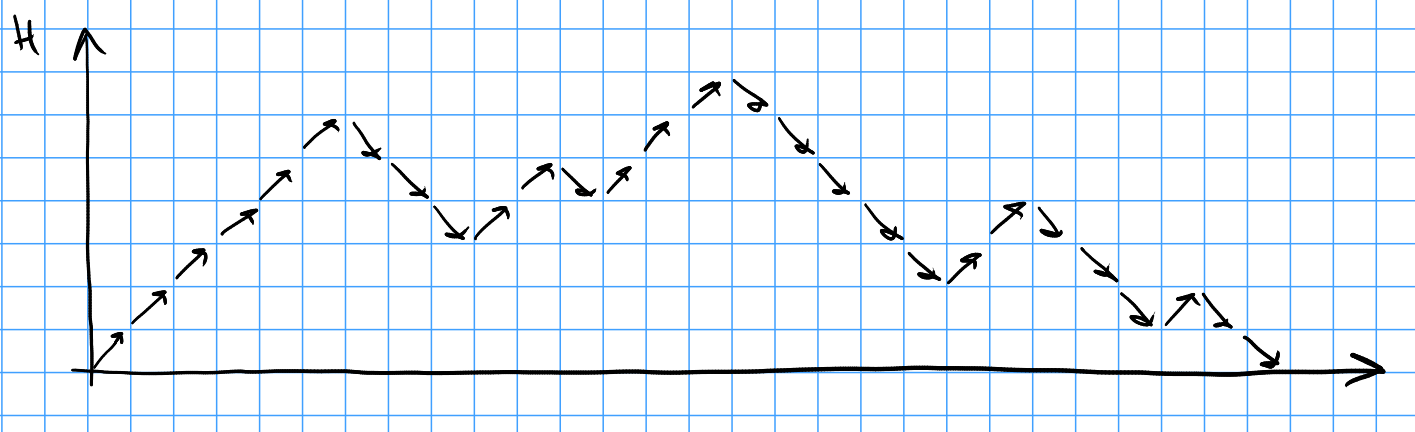
\includegraphics[width=1\linewidth]{img/dyck1_example/phase0}} 0 итерация
    \end{minipage}
    \hfill
    \begin{minipage}[h]{0.47\linewidth}
        \center{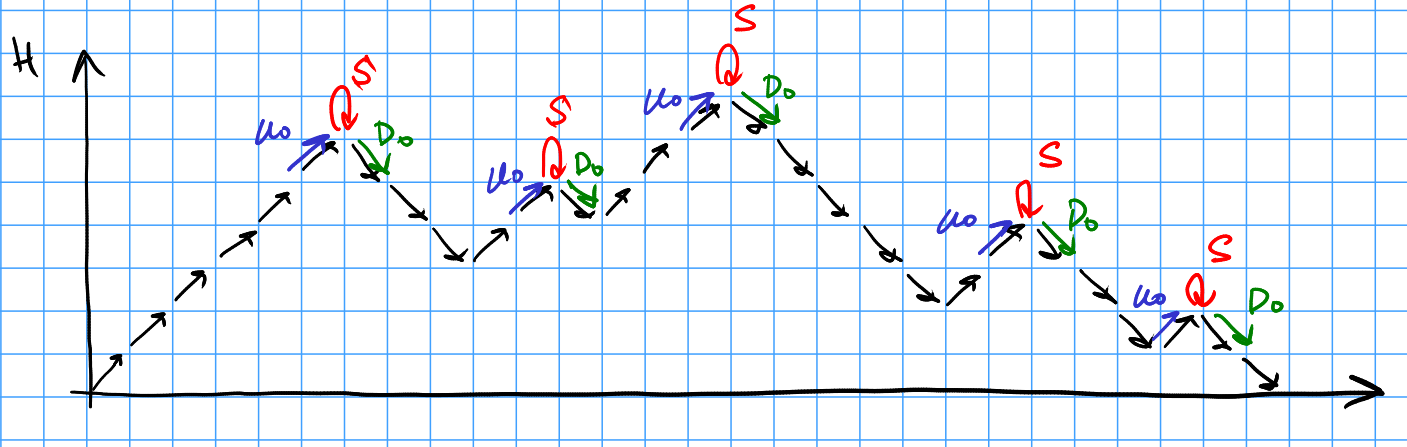
\includegraphics[width=1\linewidth]{img/dyck1_example/phase1}} 1 итерация
    \end{minipage}
    \vfill
    \begin{minipage}[h]{0.47\linewidth}
        \center{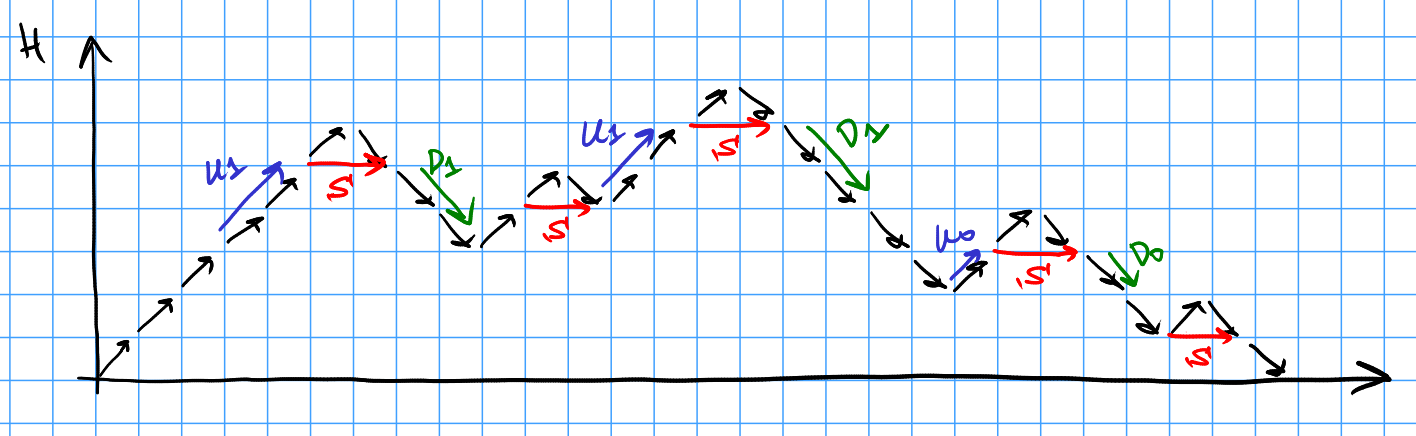
\includegraphics[width=1\linewidth]{img/dyck1_example/phase2}} 2 итерация
    \end{minipage}
    \hfill
    \begin{minipage}[h]{0.47\linewidth}
        \center{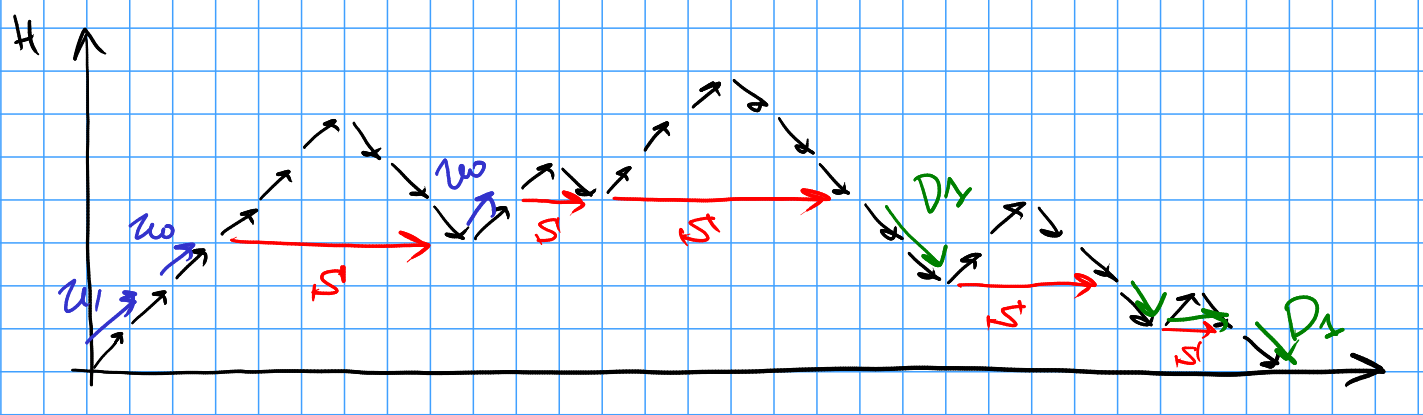
\includegraphics[width=1\linewidth]{img/dyck1_example/phase3}} 3 итерация
    \end{minipage}
    \vfill
    \begin{minipage}[h]{0.47\linewidth}
        \center{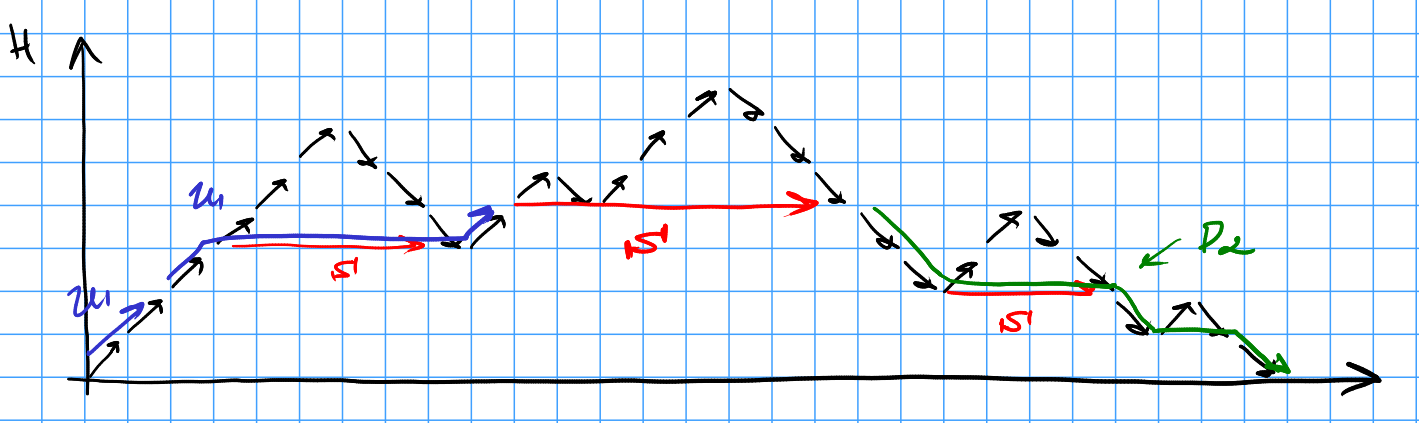
\includegraphics[width=1\linewidth]{img/dyck1_example/phase4}} 4 итерация
    \end{minipage}
    \hfill
    \begin{minipage}[h]{0.47\linewidth}
        \center{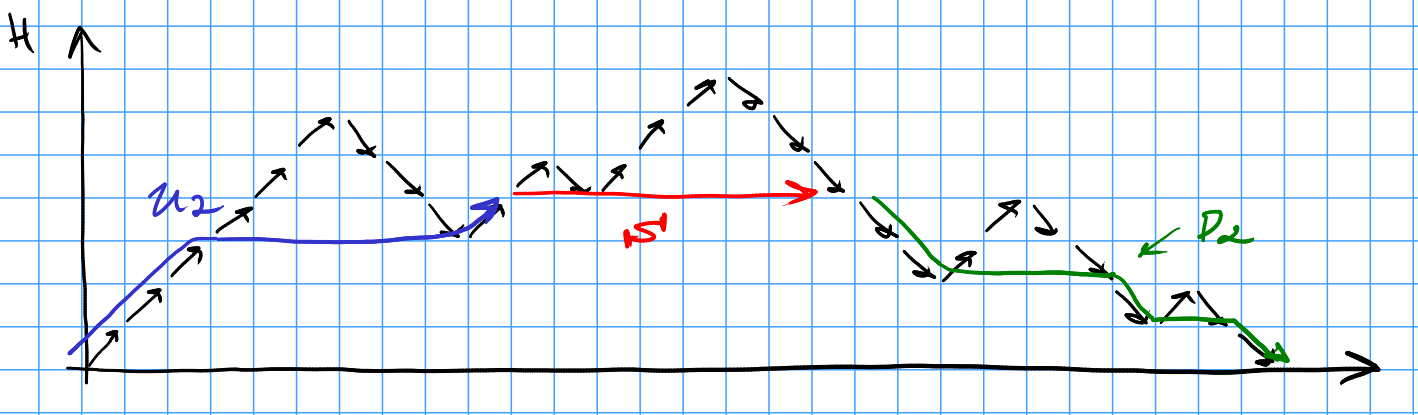
\includegraphics[width=1\linewidth]{img/dyck1_example/phase5}} 5 итерация
    \end{minipage}

    \caption{Пример работы алгоритма (на конкретном пути)}
    \label{img:dyck1_example}
\end{figure}

\TODO: норм картиночька

\subsubsection{Корректность алгоритма}

Посмотрим на нетерминал $S$ (опр.~\ref{eq:S}). В нём присутствуют все продукции из стандартного вида грамматики для языка $\cool{D}_1$, так что нужно доказать лишь, что все строки, которые выводятся остальными продукциями тоже являются корректными.

\TODO

\subsubsection{Время работы}

\TODO: \textit{Я сейчас докажу $\O(n^{\omega} \log^3 n)$, но, кажется, можно сократить на лог (засчёт того, что у нас параллельно сжимаются и $S$-ки, и $U$-шки с $D$-шками)}

Для доказательства времени работы нам потребуется пара вспомогательных утверждений.

\begin{lemma}
    После $i$-ой итерации алгоритма 
\end{lemma}

\begin{theorem}
Время работы Алгоритма (link (?)) на языке Дика на одном типе скобок~--- $\O(n^{\omega} \log^3 n)$, где $n$~--- число вершин входного графа.
\end{theorem}

\begin{proof}
Время работы алгоритма П состоит из двух множителей: времени работы одной итерации и числа итераций.

Время работы одной итерации в алгоритме П составляло $\O(N^{\omega})$ (где $N$~--- число состояний РКА-произведения), т.к. на каждой итерации считалось транзитивное замыкание. Заметим, что на самом деле достаточно находить транзитивное замыкание отдельно в каждой компоненте РКА (т.к. разные компоненты вообще не связны). Т.к. компоненты РКА грамматики константны, то размер компонент РКА-произведения~--- $\O(n)$. Так что суммарное время работы одной итерации составит $\O(n^{\omega} K)$.   
% (\TODO: link)~---\\ $O(\langle \text{время работы одной итерации} \rangle \cdot \langle \text{\# итераций} \rangle)$.

Оценим теперь число итераций. 

\TODO: \textit{за лог итераций срезаются все уголки (локальные максимумы), нужно теперь их аккуратно посчитать, смотря на соседей (и минимумы)}

\end{proof}

\begin{note}
Этот результат, скорее всего, не обобщается на языки Дика с большим типом скобок. 

Мотивация примерно такая: во1, они сложнее (язык Дика на $\ge 2$ типах скобок~--- такой же мощный как и произвольный КС-язык (теорема Хомского-Шутценбергера, тогда как язык Дика на одном типе скобок вроде как попроще. \textit{Ещё Дик на $\ge 2$ типах скобок генерирует full AFL (Abstract Families of Languages) (что бы это не значило)}), во2, сейчас мы играли на том, что состояние~--- примерно одна чиселка (ну опять-таки, язык Дика на одном типе скобок распознаётся автоматом с одним счётчиком), а для большего типа скобок нужен весь стек.
\end{note}

\subsection{Выводы и результаты по главе}